% !Mode:: "Tex:UTF-8"
\chapter{结构感知的CNF混淆算法}
\label{chap:3}

\section{引言}%
软硬件设计验证过程中,通过Tsentin编码\cite{Tseitin}将硬件电路、软件代码及待验证属性转化为统一的CNF
%(Conjunctive Normal Form)
公式,并进行SAT求解,以判断系统是否符合要求。
SAT求解问题是面向位级的,解空间随软硬件系统规模成指数级增长,对计算能力的扩展性要求高,适合部署在能够提供弹性计算资源的开放环境下。
但是,虽然电路在Tsentin编码过程中损失了很多有用的逻辑信息,研究表明,编码后生成的CNF公式中仍然携带了硬件电路结构等敏感信息;另一方面,由于SAT问题的结果反映待验证属性是否符合预期,直接影响设计方案的成败,因此错误结果也是不可容忍的。

为避免开放环境下可能出现上述问题,本章以电路设计验证中SAT问题为研究对象,对系统进行建模,分析其中存在的安全威胁,在此基础上提出了基于CNF 混淆的安全可验证SAT求解方法,在从理论上证明混淆算法的正确性之后,选取ISCAS89中典型电路验证中的SAT问题,对算法进行了性能测试和评估。
\section{问题描述}
本节将以云计算环境为例来建立开放环境下SAT求解的系统模型,并分析其中的安全威胁。
\subsection{系统假设}

在本章的研究中,存在两种类型的云,私有云和公共云。私有云是可信的,但计算及存储能力受限,适合处理简单计算;
公共云可以提供弹性计算和存储资源,适合承担复杂计算任务。
CNF公式将在私有云中产生,SAT求解器部署在公共云,用于求解CNF公式,并将结果返回给私有云。
在本章的研究中,假设公共云环境下有“诚实但好奇”的计算参与者,
他们会尽力完成所有的计算任务以便获得正确的CNF公式的解,
但是它们也试图从CNF公式或解中获得他们需要的信息,例如电路结构信息。

文献\cite{csLiequivalency,csOstrowski,csRoy,csFu}
研究了抽取和利用CNF公式中电路结构信息的方法。
Roy等人\cite{csRoy}和Fu等人\cite{csFu}给出了基于子图同构以及模式匹配的电路结构抽取算法,
并能最大限度的恢复出CNF公式中的电路结构。这些技术可能会被潜在的攻击者利用来抽取敏感的电路结构信息。
因此,CNF公式包含的结构信息应该被当做隐私加以保护。

\section{基于CNF混淆的SAT求解方法}

\subsection{SAT求解框架}
设计基于开放环境下SAT求解框架,将考虑下面三个因素:

\begin{enumerate}
 \item 可移植性:目前的SAT求解器集成了冲突检测等高效机制,因此我们希望可以将其作为黑盒直接使用,
 而不是像\cite{OBfuscationd-CNFs}试图使用新的求解算法。
 \item \label{3:g2} 隐形性\cite{obfuscationBible}:求解框架应该可以保护CNF公式中的电路结构不会被获取。
\item 结果可验证:计算结果可以通过抽样的方式验证。
 \item \label{3:g3} 开销:框架不应该引入太多的开销。
\end{enumerate}

根据上述目标,
本章给出了安全可验证的SAT求解框架,该框架基于CNF公式混淆算法。
为了混淆CNF公式,
根据后续章节介绍的SSH规则策略,
采用随机的方式在CNF公式的子句中加入新的文字,并根据加入的文字在公式中构造新的子句。
新加入的文字和一部分新的子句来自于被称为单一Husk公式(见定义\ref{3:Singular-Husk-formula-definition})的噪音公式。
SSH规则保证原始的CNF公式可以和单一Husk公式无缝地混合在一起,达到\ref{3:g2}) 和 \ref{3:g3})的要求。
%SSH规则和CSA策略将在\textit{\ref{3:embeded rules})} 和 \textit{\ref{3:embeded strategy})} 小节中介绍。

\begin{definition}[单一Husk公式]\label{3:Singular-Husk-formula-definition}
单一Husk公式是仅有一个可满足解的CNF公式,
并且解中变量的赋值是非特异的,也就是不是全$T$或全$F$。
\end{definition}

框架的详细实现在图 \ref{3:fig_cldSAT}中给出。在框架下, SAT问题的求解包含了4步。\\
$\textbf{步骤 1}$, 产生器产生一个单一Husk公式$F_H$和它的一个解$R_H$。\\
$\textbf{步骤 2}$, 混淆器将原始CNF公式$F_C$和单一Husk公式$F_H$混合,并产生一个新的CNF公式$F_O$。\\
$\textbf{步骤 3}$, $F_O$由位于公共云上的SAT求解器求解,并返回结果$S_O$。\\
$\textbf{步骤 4}$, 映射器从$S_O$中抽取出$S_C$,验证器确认$S_C$是$F_C$的解。
\begin{figure}
\footnotesize\centering
\centerline{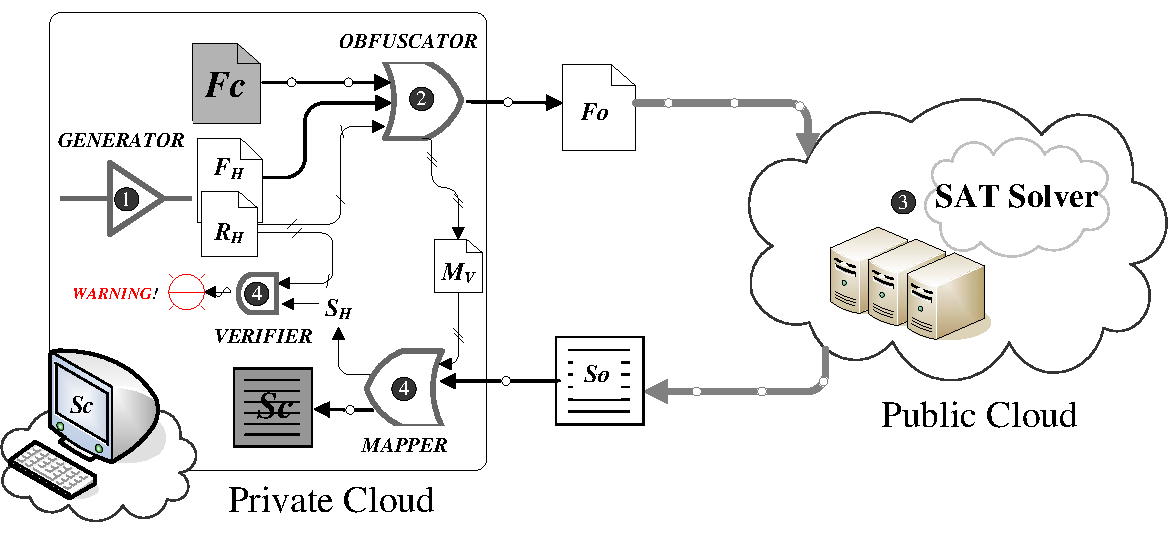
\includegraphics[width=12.2cm]{fig301}}
\caption{基于CNF公式混淆的安全可验证SAT求解框架}
%\caption{Privacy-preserving SAT solving framework based on CNF formula obfuscation.}
\label{3:fig_cldSAT}
\end{figure}

\textbf{步骤3}在公共云中运行,其余的步骤在可信的私有云上运行。
%
产生器,混淆器,映射器和验证器算法将在\ref{3:genhusk}, \ref{3:obfuscating}和\ref{3:mappping} 小节中分别介绍。
\subsection{单一Husk公式产生算法}\label{3:genhusk}

产生可满足CNF公式的算法有多种\cite{microgenSAT,genSAT},
仅有一个可满足解的单一Husk公式(见定义\ref{3:Singular-Husk-formula-definition})采用质因数的方法构造\cite{genSAT},
其中的具体实现在算法一\ref{3:algo2_genSAT}中描述。

\textbf{首先},
给定质数$p_A$(第 \ref{3:primenumber}行),
% represented by a binary vector $p_A = <a_1,a_2,\dots,a_n>$, $p_B = <b_1,b_2,\dots,b_n>$,
将$p_A \cdot p_A$ 赋值给乘法器$M$的输出,并且限制$I_1\ne 1$ and  $I_2\ne 1$ (第\ref{3:multiplePrime}行)。
其中,$I_1$和$I_2$ 是$M$的输入。

\textbf{第二},
将乘法器$M$编码为CNF公式$Tseitin(M)$(第\ref{3:TseitinPHI}行)。

为了满足$Tseitin(M)$, $M$的两个输入一定是$\{I_1=p_A,I_2=p_A\}$,
这就使得$p_A|p_A$ 为$Tseitin(M)$的解。
取$R_H=p_A$。

%
 \begin{algorithm}[t]
 \caption{GENERATOR}
 \label{3:algo2_genSAT}
 \begin{algorithmic}[1]
 \STATE input : NULL;
 \STATE output : Husks CNF $F_H$ and Husks result $R_H$;
 \STATE Generating prime numbers $p_A$; \label{3:primenumber}
 \STATE $\Phi= M(I_1 \neq 1, I_2\neq 1, O=p_A*p_A)$ ;\label{3:multiplePrime}
 \STATE $F_H=Tseitin(\Phi)$ ;\label{3:TseitinPHI}
 \STATE $R_H=p_A\mid p_A$ ;
 \end{algorithmic}
 \end{algorithm}

\subsection{解空间等价混淆算法}\label{3:obfuscating}


\subsubsection{解空间保持规则}
%To prevent information carried by CNF formula and its solution from leakage, a privacy-preserving scheme is proposed,
%the scheme is based on the following facts and anticipations:
%\\$\textbf{Fact 1:}$ Changing CNF signature and key clause in CNF formula will make circuit recovering
%based on pattern matching or subgraph isomorphism impossible.
%\\$\textbf{Fact 2:}$ Solution space should not be under-approximated after obfuscation, otherwise the result will be misleading even for real user.
%\\$\textbf{Anticipation 1:}$ According to Fact 2, solution space have to be over-approximated  after obfuscation, so as to mislead hoarding participants in public Cloud.
%\\$\textbf{Anticipation 2:}$ The solution of obfuscated CNF formula should be easily mapped back to the original formula.
%为了防止CNF公式以及解的信息泄露,给出了一个隐私保护的策略,该策略基于下面的事实和期望:
%\\$\textbf{事实 1:}$ 改变公式中的CNF标记和关键子句可以使基于模式匹配或子图同构的电路结构恢复技术失效。
%\\$\textbf{事实 2:}$ 混淆后的解空间不应该被缩小,否则会误导真实应用,例如验证等。
%%\\$\textbf{期望 1:}$ 鉴于事实2, 解空间应该被扩大,以便于误导公共云上包括SAT求解器在内的第三方。
%\\$\textbf{期望 1:}$ 可以从混淆后的解中较快的恢复出原公式的解。

本章介绍的混淆器,会通过解空间保持(SSH)规则,
将Husks公式$F_H$嵌入到原始公式$F_C$中,产生一个新的CNF公式$F_O$。
遵循SSH规则,混淆器在原公式加入新的文字或是子句,改变子句的文字集合以及公式中的子句集合,
来防止攻击者通过模式识别或是子图同构技术获取公式中携带的电路结构信息;
SSH规则同时还将保证混淆后的解空间与原公式解空间等价。

%本章在\textit{\ref{3:embeded rules}})介绍SSH规则。
%\subsubsection{解空间保持(SSH)规则}\label{3:embeded rules}
先来考虑一个有趣的问题,将SAT问题编码为CNF公式外包到云中,由SAT求解器求解;
并且不希望SAT求解器知道实际的SAT问题是怎样的。
一个简单的方法就是将真实的CNF公式和一个在变量上和其无交集的可满足公式,简单的排列混合在一起,
并将混合后的CNF公式外包的云上,
由于可满足公式必然存在解,那么如果真实公式有解,其解将会混杂在混合后的解中。
这种方法非常简单易行,
但是,基于分区\cite{Partition}的方法可以将两个不相关的公式分离开来,从而得到真实的CNF公式。

再来考虑一个改进的方法:
任意公式$F_C$,和一个可满足公式$F_H$及其唯一解\textsl{${\textbf{R}}_{\textbf{H}}$},
$F_C$和$F_H$没有公共变量, 也即:$V_{F_C}$ $\cap$ $V_{F_H}$ =$\phi$。
将$F_C$和$F_H$无缝混合,以便于隐藏$F_C$。
同时,保持$F_C$中的所有解都包含在新的公式中。

为实现$F_C$和$F_H$无缝混合,
直觉的方法是将$F_H$中的变量加入到$F_C$的子句中,
并且使用$F_C$和$F_H$中的变量产生新的子句。
根据CNF公式的定义可知其具有如下特性,对任意CNF公式$F_C$,在子句中加入新的文字可能会扩展解空间,
而加入包含$F_C$中变量的子句则会缩减解空间。
那如何在此情况下保证$F_C$所有的解仍旧保留在新的公式中?
在给出具体答案之前,首先澄清下面的概念。

\begin{definition}[解包含关系 $S_C \subseteq S_O$]~
CNF 式$F_C$和$F_O$具有$n_{F_C}$公共变量$x_1,...,x_{n_{F_C}}$ 并且有
$|V_{F_C}|\equiv n_{F_C}$, $|V_{F_O}|\equiv n_{F_O}$, $ n_{F_O}\geqslant n_{F_C} > 0$。
$S_C$和$S_O$分别是$F_C$和$F_O$的解,
在$S_C$和$S_O$中,$n_{F_C}$个公共变量的赋值是相同的, 也就是
$S_C=\{x_1=B_1,...,x_{n_{F_C}}=B_{n_{F_C}} | B_i \in \{T,F\},~1\leqslant i\leqslant n_{F_C} \}$,
$S_O=\{x_1=B_1,...,x_{n_{F_C}}=B_{n_{F_C}},...,x_{n_{F_O}}=B_{n_{F_O}}|B_i\in \{T,F\},~ 1\leqslant i\leqslant n_{F_O} \}$。
称解$S_C$包含于$S_O$,记为$S_C\subseteq S_O$。
\end{definition}

\begin{definition}[解空间等价(SSE)]\label{3:SSEdefinition}~
CNF公式$F_C$有$n$个解$\{S_{C_1},...,S_{C_n}\}$;
CNF公式$F_O$也有$n$个解$\{S_{O_1},...,S_{O_n}\}$,
并且对于任意$i \in [1,n]$, $S_{C_i} \subseteq S_{O_i}$。
称$F_O$解空间等价于$F_C$,记为$F_C \equiv_{_{SSE}} F_O$。
\end{definition}

为了在新公式中保持$F_C$公式中的所有解,
给出了解空间保持(SSH)规则,使用公式$F_H$和它的解$R_H$来混淆公式$F_C$,
以便于保证混淆后公式具有上估计的解空间。

\textbf{解空间保持(SSH)规则: }
\begin{enumerate}
\item \textbf{规则 1}:
对任一子句$c\in F_{C}$,
从$R_H$中任取出变量,
并按照下列规则插入到子句$c$:
如果在$R_H$中变量的赋值是$T$,作为负文字;
如果在$R_H$中变量的赋值是$F$,作为正文字;
用新生成的子句代替原始子句$c$。
\item \textbf{规则 2}:
使用$R_H$中的文字和$F_C$中的变量创建新的子句,按照下列规则:
如果在$R_H$中文字是$T$,就作为正文字;
如果在$R_H$中文字是$F$,就作为负文字。
\end{enumerate}


\begin{definition}[${\textbf{Obf(}}F_C,F_H,R_H\textbf{)}$]\label{3:OBFUSCATORSSH}
对任意公式$F_C$, 和可满足公式$F_H$及其一个赋值$R_H$,

$Obf(F_C,F_H,R_H)$ 是在基于SSH规则将$F_C$和$F_H$混合后得到的公式。

如果$F_H$是单一Husk公式并且$R_H$是它的唯一解,
就称$Obf(F_C,F_H,R_H)$为解空间等价的混淆,简称为${\textbf{SSE obfuscation}}$。

%如果$F_H$是Husks公式并且$R_H$是它其中一个解, 就称$Obf(F_C,F_H,R_H)$为${\textbf{SSO obfuscation}}$。
\end{definition}
% \begin{definition}[${\textbf{Obf(}}F_C,F_H,R_H\textbf{)}$]\label{3:OBFUSCATORSSH}
% For arbitrary formula $F_C$, and satisfiable formula $F_H$ with $R_H$ as one of its solutions,
% $Obf(F_C,F_H,R_H)$ is the result of applying SSH Rules when blending $F_C$ with $F_H$.
% If $F_H$ is a Singular Husk formula, $Obf(F_C,F_H,R_H)$ is called ${\textbf{SSE obfuscation}}$.
% If $F_H$ is Husks formula, $Obf(F_C,F_H,R_H)$ is called ${\textbf{SSO obfuscation}}$.
% \end{definition}

%For SSH based obfuscation, we have following theorems.
对基于SSH规则的${\textbf{SSE obfuscation}}$,下列定理成立。

\begin{theorem}[SSE Obfuscation]\label{3:SSEtheorem}

对任意CNF公式 $F_C$,和单一Husk公式$F_{_SH}$,如果

~~$V_{F_C}$ $\cap$ $V_{F_{_SH}}$ =$\phi$, 并且
$R_{_SH}$是$F_{_SH}$的唯一解,

则 $Obf(F_C,F_{_SH},R_{_SH}) \equiv F_C\wedge F_{_SH}$。
\end{theorem}

基于定理\ref{3:SSEtheorem}和定义\ref{3:SSEdefinition},有:
% inference \ref{3:SSEinference}.
%\begin{inference}\label{3:SSEinference}
\begin{theorem}\label{3:SSEinference}
对任意CNF公式 $F_C$,和单一Husk公式$F_{_SH}$,如果

~~$V_{F_C}$ $\cap$ $V_{F_{_SH}}$ =$\phi$, and
$R_{_SH}$是$F_{_SH}$的唯一解,

则 $Obf(F_C,F_{_SH},R_{_SH}) \equiv_{_{SSE}} F_C$。
\end{theorem}
%\end{inference}

%Theorem \ref{3:SSEtheorem} and \ref{3:SSOtheorem} will be proved in Subsection \ref{3:correctness}.
%An obfuscated CNF formula $F_O=Obf(F_C,F_H,R_H)$ generated by SSO obfuscation
%consists of all the variables of $F_C$ and $F_H$.

经过SSE混淆生成的CNF公式$F_O=Obf(F_C,F_{_SH},R_H)$,包含了$F_C$和$F_{_SH}$中的所有变量;
并且根据SSH\textbf{规则1},$F_C$中的部分子句被加入了$F_{_SH}$中的变量文字而成为了新的子句,
由于$F_{_SH}$解的非特异性,这些文字不全为正也不全为负;
还有部分子句是根据SSH\textbf{规则2},由分别取自$F_C$和$F_{_SH}$的变量文字组合而成的;
从形式上看,$F_O$是一个合法并且普通的CNF公式。
而根据定理\ref{3:SSEtheorem},可知混合后公式$F_O$的解是$F_C$和$F_{_SH}$的交集,
由于公式$F_C$和$F_{_SH}$无公共变量,又由于$F_{_SH}$只有唯一解;
这就使得$F_O$的解的个数和$F_C$的一致,可以得到如下的结论:

%$F_H$中的变量被赋值为$R_H$,则有:
%
%$F_O(R_H/V_{F_O})
%=Obf(F_C,F_H(R_H/V_{F_H}),R_H)$
%
%根据引理\ref{3:SHE}(\ref{3:correctness}小节),
%$F_H(R_H/V_{F_H})$可以被表示为一个单一Husk公式,有唯一解$R_H$。
%根据推论\ref{3:SSEinference},对任意$F_C$和混淆后公式$F_O$,则有:
\begin{enumerate}
 \item $F_C$是不可满足的当且仅当$F_O$不可满足,
 并且 $F_C$的不可满足核可以通过从$F_O$的不可满足核中删除$F_H$中的文字获得。
 \item $F_C$可满足当且仅当$F_O$是可满足的,
 并且$F_C$的解可以通过将$F_O$的解投影到$F_C$的变量集中获得。
\end{enumerate}

如果$F_C$有解,$F_O$的解可以被划分为$F_C$和$F_H$的解;
$F_C$的解可以从$F_O$的解中通过投影获得。

综上所述,经过SSH混淆变换后,
$F_O$和$F_C$在形式上相似,$F_O$和$F_C$可以使用同样的SAT求解器求解,
在不知晓$R_H$的情况下,$F_C$将很难从$F_O$剥离;
另一方面,$F_O$的解空间和$F_C$解空间等价。
通过SSH规则,OBFUSCATOR可以在子句中添加新文字并且创建新的子句,同时保证解空间不被扩展或缩减;
这实现了对SAT求解同构加密的混淆效果。

定理\ref{3:SSEtheorem}的严格证明将在\ref{3:correctness}小节给出。
\subsubsection{\textsl{OBFUSCATOR算法}}

OBUFSCATOR算法遵循上述SSH规则,混淆CNF公式$F_C$,从而防止$F_C$的携带的电路结构信息被潜在的攻击者获取。
SSH规则保证了解空间的不变,如何达到隐藏电路结构信息的目的,则需要确定如何在子句中添加新的文字以及构造新的子句。

为了达到上述目标,OBFUSCATOR首先会标记CNF公式中的关键子句,以确定究竟选取哪些子句加入文字;
而后通过在关键子句中加入噪音文字,破坏原有的结构。
OBFUSCATOR的详细实现在算法\ref{3:algo_obs}中,
其中使用$mark$(第$\ref{3:mark}$行)来检测CNF公式中的关键子句和输出变量,
并使用$generate\_new\_clause$(第$\ref{3:gennewclause}$行)产生新的子句。

由于AND2是最常见的门,
在仅仅给出AND2门的$\mathbf{mark}$算法,
同样,也仅仅给出AND2的$\mathbf{generate\_new\_clause}$算法,
这两个算法组合起来可以将AND2的标记转换为AND3的标记。具体的实现在算法\ref{3:algo_mark}中。

\begin{algorithm}[t]
\caption{OBFUSCATOR}
\label{3:algo_obs}
%\SetAlgoNoLine
\begin{algorithmic}[1]
\STATE input : The original CNF $F_C$, Husks CNF $F_H$, Husks result $R_H$
\STATE output : The obfuscated CNF $F_O$, variable mapping $M$
\STATE $mark(F_C)$;\label{3:mark}
\FOR{$c\in F_C$}
\IF{$c \in$  Key Clause Set } \label{3:keyclause}
\STATE     lit =get literal $ \in R_H$;
\STATE     $c=c \cup \neg lit$;\label{3:rule1}
\STATE     $nc=generate\_new\_clause(c,lit)$;\label{3:gennewclause}
 \STATE    $F_C=F_C \cup nc$;\label{3:blendclause1}
\ENDIF
\ENDFOR
\FOR{$ c \in F_C $}
\STATE $averagelen=\frac{\sigma _{c'\in F_C}|c'|}{|F_C|}$ ;
\WHILE{$|c| < averagelen$}
\STATE $lit=$get literal $\in R_H$ ;
\WHILE{$\neg lit \in c$}
\STATE lit=get literal $ \in R_H $ ;
\ENDWHILE
\STATE $c=c \cup \neg lit$;\label{3:rule1-2}
\ENDWHILE
\STATE $M$ =remap all variable in $F_C\cup F_H$ ;\label{3:MV}
\STATE $F_O$ =reorder all clause in $F_C\cup F_H$ ; \label{3:blendclause2}
\ENDFOR
\end{algorithmic}
\end{algorithm}

\begin{algorithm}[t]
\caption{$\mathbf{mark}$ and $\mathbf{generate\_new\_clause}$}
\label{3:algo_mark}
\begin{algorithmic}[1]
%\SetAlgoNoLine
\STATE $\mathbf{mark}$;
\STATE input : CNF formula $S$;
\STATE output : marked $S$ ;
\FOR{$(C \in S) ~\&~ (|C|\equiv 3)$}
\FOR{$l \in C$ }
\FOR{$(C_1 \in S) ~\&~ (\neg l\in C_1)~ \&~ (|C_1|\equiv 2)$ }
\FOR{$l_1 \in C_1$ }
\IF{$(\neg l_1 \in C)~\&~(l_1\ne l)$}
\STATE $match++$ ;
\ENDIF
\ENDFOR
\ENDFOR
\ENDFOR
\ENDFOR
\IF{$match\equiv 2$}
\STATE mark $l$ as output literal ;
\STATE mark $C$ as Key Clause;
\ENDIF

\STATE $\mathbf{generate\_new\_clause}$;
\STATE input : key clause $C$ in AND2, Husk literal $lit$;
\STATE output : new clause $C_1$;
\STATE $olit$=Getting output literal from $C$ ;
\STATE $C_1= lit \cup \neg olit$ ;\label{3:rule2}
\end{algorithmic}
\end{algorithm}


%\begin{algorithm*}[b]
%\caption{GENERATOR}
%\label{3:algo2_gen}
%\begin{algorithmic}[1]
%%%\SetAlgoLined
%%\SetAlgoNoLine
%\STATE input : NULL
%\STATE output : Husks CNF $F_H$ and Husks result $R_H$
%\STATE Generating prime numbers $p_A$ and $p_B$  ; \label{3:primenumber}
%\STATE $\Phi= M(I_1 \neq 1, I_2\neq 1, O=p_A*p_B)$ ;\label{3:multiplePrime3MVMV}
%\STATE $F_H=Tseitin(\Phi)$ ;\label{3:TseitinPHI}
%\STATE $R_H=p_A\mid p_B$ ;
%\end{algorithmic}
%\end{algorithm*}

\subsection{映射和验证算法}\label{3:mappping}
在公共云上的求解器完成求解并给出$F_O$解$S_O$,并返回给私有云中。
和混淆器相对应,在私有云中使用MAPPER和VERIFIER将$F_C$的解从$S_O$中过滤出来。
MAPPER和VERIFIER的实现在算法\ref{3:algo_map}中。

根据定理\ref{3:SSEtheorem},
如果结果是UNSAT, 那么原始的CNF公式也是(第\ref{3:sUNSAT}行)。
如果结果是SAT, MAPPER(\ref{3:var}-\ref{3:mapper}行)将解投影到$F_C$和$F_H$的变量上,
以获得$S_C$ 和$S_H$,分别作为$F_C$和$F_H$的候选解。
VERIFIER(\ref{3:verifer1}-\ref{3:verifer2}行)检测$S_H$是否等于$R_H$,
如果等于, $S_C$就是$F_C$的真实解。
否则,$S_C$是错误解,说明云端给出的结果是不可信的。

解的投影过程依赖于变量映射表$M$,它由OBFUSCATOR(算法\ref{3:algo_obs}的\ref{3:MV}行)创建。
$M[var].variable$ (第\ref{3:var}行)表示了var的原始变量名,
$M[var].formula$ (第\ref{3:formula}行)表示var所属于的公式,可以是$F_C$ 或 $F_H$。


\begin{algorithm}[t]
\caption{MAPPER-VERIFIER}
\label{3:algo_map}
%\SetAlgoNoLine
\begin{algorithmic}[1]
% \SetAlgoNoLine
\STATE input : Obfuscated result $S_O$, variable mapping table $M$, Husk result $R_H$;
\STATE output : Result $S_C$;
\IF{$S_O$ is UNSAT} \label{3:sUNSAT}
\RETURN UNSAT ;
\ENDIF
\FOR {$lit \in S_O$}
\STATE $var=abs(lit)$;
\STATE $rvar=M[var].variable $;\label{3:var}
\IF{$M[var].formula ~is~ F_C$}  \label{3:formula}
\STATE $S_C[rvar]=lit>0?rvar:\neg rvar$ ; \label{3:mapper}
\ELSE
\STATE $Hlit=lit>0?rvar:\neg rvar$;\label{3:verifer1}
\IF{$R_H[rvar]\ne Hlit$}
\STATE    alert("Something wrong with Solution!!! "); \label{3:Warning}
\STATE    break;
\ENDIF
\ENDIF
\label{3:verifer2}
\ENDFOR
\PRINT " SAT  solution is $S_C$ ";
\caption{MAPPER and VERIFIER}
%\label{3:algo_map}
\end{algorithmic}
\end{algorithm}
\section{理论分析和实验评估}
\subsection{理论分析}
\subsubsection{正确性证明}\label{3:correctness}
根据定理\ref{3:SSEtheorem},在SSH规则下,
原始的CNF公式可以和Husks公式无缝混合, 而不会改变解空间。
在本节中,证明这一定理。
在此之前,首先给出SSH混淆过程逻辑步骤描述和相关引理,这是定理证明的基础。

算法\ref{3:algo_obs}实现的基于SSH规则的混淆过程,
从逻辑上看分为如下三步,描述如下:
% \textbf{SSO obfuscation with SSH rule and CSA strategy}
%\begin{procedure}[${Obf_{SSH\_CSA}}$]\label{3:obsprocedure}~

\textit{\textbf{Procedure \ref{3:obsprocedure}}}.
\begin{enumerate}
\item[]\label{3:obsprocedure}
输入:公式$F_C$, 单一Husk公式$F_H$, 解$R_H$.
(其中$F_C$包含了\textbf{关键子句}(第\ref{3:keyclause}行)和\textbf{非关键子句},
相应的子句集合表示为\textbf{$F_{Ck}$}和\textbf{$F_{Cn}$}.)
\item[] 输出: 公式 $F_O$.
\end{enumerate}

\textbf{步骤1}:
对关键子句$c\in F_{Ck}$,
从$R_H$中取出文字$lit$,根据SSH规则1
将$\neg lit$加入到$c$(算法\ref{3:algo_obs}的\ref{3:rule1}, \ref{3:rule1-2}行).
生成子句的集合记为$S_3$ .

\textbf{步骤2}:
根据SSH规则2,
使用$R_H$中文字lit和$c$中的输出变量,产生新的子句(算法 \ref{3:algo_obs}的\ref{3:gennewclause}行,  算法\ref{3:algo_mark}的\ref{3:rule2}行)。

新产生的子句集合记为$S_4$.

\textbf{步骤3}:
将$S_3$, $S_4$, $F_H$, 和$F_{Cn}$, 混合产生$F_O$ (算法\ref{3:algo_obs}的\ref{3:rule1}, \ref{3:rule1-2}, \ref{3:blendclause1} \ref{3:blendclause2} 行).

\textit{\textbf{end Procedure}}.


\begin{lemma}[Singular Husk Equation(SHE)]\label{3:SHE}

对单一Husk公式${F_H}$且有$|V_{F_H}|= n$,
其唯一解$S_H$=$\{(y_i=B_i,y_j=B_j)|B_i\equiv T, B_j\equiv F, 1\leqslant i, j\leqslant n \}$.

令$F_{_SH}=F_H\wedge (\bigwedge_{1\leqslant i\leqslant n}^{B_i\equiv T}y_i)\wedge(\bigwedge_{1\leqslant j\leqslant n}^{B_j\equiv F}\neg y_j)$

\textbf{则有} $F_H \equiv F_{_SH}$.
\end{lemma}
\begin{proof}~\\
1)因为$F_H\equiv T$, $F_H$有唯一解$S_H$。
 \begin{equation}\label{3:S_H}
 S_H=\{(y_i=B_i,y_j=B_j)|B_i\equiv T, B_j\equiv F, 1\leqslant i, j\leqslant n \}.
\end{equation}
根据式\ref{3:S_H}),构造$F_{_{lS}H}$
\begin{equation}
 F_{_{lS}H}=(\bigwedge_{1\leqslant i\leqslant n}^{B_i\equiv T}y_i)\wedge(\bigwedge_{1\leqslant j\leqslant n}^{B_j\equiv F}\neg y_j)
\end{equation}
则有
\begin{equation}
 F_{_{lS}H} \equiv T
\end{equation}
构造$F_{_SH}$
\begin{equation}
 F_{_SH}=F_H\wedge F_{_{lS}H}
\end{equation}
则有
\begin{equation}
 F_{_SH} \equiv T
\end{equation}
\begin{equation}
 F_H \vdash F_{_SH}
\end{equation}\\
2)因为 $F_{_SH}\equiv T$
\begin{equation}
F_{_SH}=(\bigwedge_{1\leqslant i\leqslant n }^{B_i\equiv T}y_i)\wedge(\bigwedge_{1\leqslant j\leqslant n}^{B_j\equiv F}\neg y_j)
\end{equation}
则有$F_{_SH}$的唯一解$S_H$
\begin{equation}
S_H=\{(y_i=T,y_j=F)|B_i\equiv T, B_j\equiv F, 1\leqslant i, j\leqslant n \}
\end{equation}
令 $B_i$替换$T$, $B_j$替换$F$,则有
 \begin{equation}
S_H=\{(y_i=B_i,y_j=B_j)|B_i\equiv T, B_j\equiv F, 1\leqslant i, j\leqslant n \}
 \end{equation}
因为$S_H$是$F_H$的解, 则有
\begin{equation}
F_H(S_H/V_{F_H})\equiv T
\end{equation}
 因此有
 \begin{equation}
  F_H \vdash F_{_SH}
 \end{equation}
 \\
因为 1) and 2):
\begin{equation}
 F_H \equiv F_{_SH}.
\end{equation}
\end{proof}

根据引理\ref{3:SHE},一个单一Husk公式等价于解文字的合取。

%\begin{lemma}[OR Hold Obfuscation]\label{3:ORrelation-Holding-Obfuscation}
%对公式$F_C$ 和$F_{_RH}\vee F_{_SH}$,及$F_{_RH} \vee F_{_SH}$的一个赋值$R_H$ 有,
%
%$Obf(F_C,F_{_RH}\vee F_{_SH},R_H)\equiv Obf(F_C,F_{_RH},R_H) \vee Obf(F_C,F_{_SH},R_H)$
%\end{lemma}
%\begin{proof}
%假设:
%\begin{enumerate}
% \item[-]$F_C$=$F_{Ck} \wedge F_{Cn}$,  $F_{Ck}$= $\bigwedge_{1}^{m}(a_i\vee X_i$).
% \item[-]$F_H$=$F_{_RH}\vee F_{_SH}$
% \item[-]$R_H$=$\{y_j=B_j| B_j \in \{T,F\}, 1\leqslant j\leqslant n\}$.
% \item[-]令 $F_O=Obf(F_C,F_H,R_H)$
% \end{enumerate}
%% \begin{enumerate}
%% \item[-] Clause $A=a\vee X$,and clause $B=b$, while $b\notin X$,arbitary formula $F_{Cn},F_{_SH}$
%% \item[-] Let $F_{Ck} =A, F_C=F_{Ck} \wedge F_{Cn}$, $F_{_RH}=B$ $F_H=F_{_RH}\vee F_{_SH}$, while $R_H=\{b\equiv T\}$;
%% \item[-] Let $F_O=Obf(F_C,F_H,R_H)$
%% \end{enumerate}
%%  ~~~~then $F_O=(F_C\wedge F_H) \vee Obf(F_C,F_{_SH} ,R_H$
%根据\textbf{Procedure}\ref{3:obsprocedure},按下列3个\textbf{步骤}构造$F_O$.
%\begin{enumerate}
%\item  $(y_j\equiv B_j)\in$ $R_H$, $(a_i\vee X_i) \in F_{Ck}$和规则1:
%\begin{itemize}
% \item[] 如果$B_j\equiv T$, 则子句$C_{ij}=(a_i\vee X_i)\wedge \neg y_j$.
% \item[] 如果$B_j\equiv F$, 则子句$C_{ij}=(a_i\vee X_i)\wedge y_j$.
%\end{itemize}
%令$S_3=\bigwedge_{1\leqslant i\leqslant m}^{1\leqslant j\leqslant n} C_{ij}$
%\item
%$(y_j\equiv  B_j)\in $ $R_H$, $(a_i\vee X_i) \in F_{Ck}$以及规则2:
%\begin{itemize}
% \item[] 如果$B_j\equiv T$, 则子句$D_{ij}=\neg a_i\wedge y_j$.
% \item[] 如果$B_j\equiv F$, 则子句$D_{ij}=\neg a_i\wedge \neg y_j$.
%\end{itemize}
%令$S_4=\bigwedge_{1\leqslant i\leqslant m}^{1\leqslant j\leqslant n} D_{ij}$.
%\item\label{3:ORFO}
%令$F_{_dC} =S_3\wedge S_4 \wedge F_{Cn}$, then $F_O=F_H \wedge F_{_dC}$.
%\end{enumerate}
%根据步骤\ref{3:ORFO}):
%\begin{equation}\label{3:FOOBF}
%\begin{array}{ccc}
%F_O  =  F_H \wedge F_{_dC}                                   &F_H=F_{_RH}\vee F_{_SH}&\models\\
%F_O  =  (F_{_RH}\vee F_{_SH})\wedge F_{_dC}                  &                       &\models\\
%F_O  =  (F_{_RH} \wedge F_{_dC})\vee(F_{_SH}\wedge F_{_dC})  &                       &
%\end{array}
%\end{equation}
%根据\textbf{Procedure}\ref{3:obsprocedure}, $F_{_dC}$仅和$F_C$以及$R_H$相关, 则\\
%% \begin{equation}
%%  Obf(F_C,F_H,R_H) \equiv F_H \wedge F_{_dC}
%% \end{equation}
%\begin{equation}\label{3:SHOBF}
%F_{_SH} \wedge F_{_dC} \equiv Obf(F_C,F_{_SH},R_H)
%\end{equation}
%\begin{equation}\label{3:RHOBF}
%F_{_RH} \wedge F_{_dC} \equiv Obf(F_C,F_{_RH},R_H)
%\end{equation}
%根据式(\ref{3:FOOBF}), (\ref{3:SHOBF}), (\ref{3:RHOBF}), 有:
% \begin{equation}
%F_O \equiv Obf(F_C,F_{_RH} ,R_H)
%\vee Obf(F_C,F_{_SH} ,R_H)
% \end{equation}
%
%%\textit{end proof.}
%\end{proof}
%
% \begin{lemma}[AND Hold Obfuscation]\label{3:ANDrelation-Holding-Obfuscation}
\begin{lemma}[AND Hold Obfuscation]\label{3:ANDrelation-Holding-Obfuscation}
公式$F_C$ 和$F_{_RH}\wedge F_{_SH}$,
并且$R_H$是$F_{_RH} \wedge F_{_SH}$的一个赋值, 则有

$Obf(F_C,F_{_RH} \wedge F_{_SH},R_H) $
$\equiv Obf(F_C,F_{_RH},R_H) \wedge Obf(F_C,F_{_SH} ,R_H)$
\end{lemma}
\begin{proof}
%\textsl{略.}
%同Lemma \ref{3:ORrelation-Holding-Obfuscation}.
 \textbf{假设}
 \begin{enumerate}
 \item[] 子句$A=a\vee X$和子句$B=b$,并且$b\notin X$,任意公式$F_{Cn},F_{_SH}$
 \item[] 令$F_{Ck} =A, F_C=F_{Ck} \wedge F_{Cn}$, \\
           $F_{_RH}=B, F_H=F_{_RH}\wedge F_{_SH}$, 并且 $R_H=\{b\equiv T\}$;
 \item[] 令$F_O=Obf(F_C,F_H,R_H)$
 \end{enumerate}
 % then $F_O=Obf(F_C,F_{_RH},R_H)\wedge Obf(F_C,F_{_SH},R_H)$.
 根据\textbf{Procedure} \ref{3:obsprocedure}, 按下列3个步骤构造$F_O$。
 \begin{enumerate}
 \item 根据$R_H$和规则1,有子句 $C=A\vee \neg b$, and $S_3=C$
 \item 根据$R_H$和规则2,并且有文字$a\in A$,有子句$D=\neg a\vee b$;我们令$S_4=D$;
 \item 令$F_{_dC} =S_3\wedge S_4 \wedge F_{Cn}$,则$F_O=F_H \wedge F_{_dC}$.
 \end{enumerate}
 \begin{equation}\label{3:ANDequation}
 \begin{array}{ccc}
 F_O  =  F_H \wedge F_{_dC}                                     & F_H=F_{_RH}\wedge F_{_SH}&\models\\
 F_O  =  (F_{_RH}\wedge F_{_SH})\wedge F_{_dC}                   &                        &\models\\
 F_O  =  (F_{_RH} \wedge F_{_dC})\wedge (F_{_SH} \wedge F_{_dC})  &                        &\models\\
 \end{array}
 \end{equation}
 根据\textbf{Procedure} \ref{3:obsprocedure}, $F_{_dC}$仅仅和$F_C$、$R_H$相关, 则
\begin{equation}\label{3:FSHequation}
 F_{_SH} \wedge F_{_dC} \equiv Obf(F_C,F_{_SH},R_H)
\end{equation}
\begin{equation}\label{3:FRHequation}
 F_{_RH} \wedge F_{_dC} \equiv Obf(F_C,F_{_RH},R_H)
\end{equation}
根据式\ref{3:ANDequation})、\ref{3:FSHequation})和\ref{3:FRHequation}),则有
\begin{equation}
 F_O  = Obf(F_C,F_{_RH},R_H)\wedge Obf(F_C,F_{_SH},R_H)
\end{equation}
\
\textit{end proof.}
\end{proof}

%根据引理\ref{3:ORrelation-Holding-Obfuscation}和\ref{3:ANDrelation-Holding-Obfuscation},
%对单一Husk公式$F_H$,  AND和OR关系在混淆后依然保持。
%%%%%%%%%%%%%%%%%%%%%%%%%%%%%%%%%%%%%%%%%%%%%%%%%%%%%%%%%%%%%%%%%%%%%%%%%%%%%%%%%%%%%%%%%%%%%%%%%%%%%%%%%%%%%%%%%%%%%%%%%%%%%%%
%\begin{lemma}[Unique Positive literal SSE Obfuscation]\label{3:UPSSE-lemma}
%% \textbf{(Unique Positive literal SSE Obfuscation)}
%For any CNF formula $F_C$, we have
%
%\textbf{$Obf(F_C,B=b,{b\equiv T})\equiv F_C\wedge b$}
%\end{lemma}
%\begin{proof}
%%\textbf{Unique Positive literal SSE Obfuscation (UPSSE)}:\label{3:UPSSE-lemma}
%Assume
%\begin{enumerate}
% \item[-]$F_C$=$F_{Ck} \wedge F_{Cn}$, $F_{Ck}=A$, $A=a\vee X$.
% \item[-]$F_H$=$B$, $B=b$~while $b\notin X$, $R_H$=$\{b\equiv T\}$.
% \item[-]Let $F_O=Obf(F_C,F_H,R_H)$
% \end{enumerate}
%% \begin{enumerate}
%% \item[-] Clause $A=a\vee X$, an arbitary formula $F_{Cn}$ and clause $B=b$, while $b\notin X$;
%% \item[-] Let $F_{Ck} =A, F_C=F_{Ck} \wedge F_{Cn}$, $F_H=B$, while $R_H=\{b\equiv T\}$;
%% \item[-] Let $F_O=Obf(F_C,F_H,R_H)$
%% \end{enumerate}
%%  ~~~~then $F_O=F_C\wedge F_H$.
%According to \textbf{Procedure} \ref{3:obsprocedure}, Construct $F_O$ as following 3 \textbf{steps}.
%\begin{enumerate}
%\item With $(b\equiv T) \in $ $R_H$ and Rule 1,
%we have clause $C=A\vee \neg b$, and $S_3=C$.
%\item
%With ($b\equiv T) \in $ $R_H$, literal $a\in A$ and Rule 2,
%we have clause $D=\neg a\vee b$,
%and $S_4=D$.
%\item \label{3:UPSSEFO}
%let $F_O=F_H \wedge S_3\wedge S_4 \wedge F_{Cn}$.
%\end{enumerate}
%According to Step \ref{3:UPSSEFO}):
%\begin{equation}
%\begin{array}{ccc}
%F_O  =  F_H \wedge S_3\wedge S_4\wedge F_{Cn}           &S_3=C~ S_4=D              &\models\\
%F_O  =  F_H\wedge C\wedge D\wedge F_{Cn}                &F_H=B~ B=b                &\models\\
%F_O  =  b\wedge C\wedge D\wedge F_{Cn}                  &C=A\vee \neg b~           &\models\\
%F_O  =  b\wedge (A\vee \neg b) \wedge D\wedge F_{Cn}    &                          &\models\\
%F_O  =  b\wedge A \wedge D\wedge F_{Cn}                 & D=\neg a\vee b~          &\models\\
%F_O  =  b\wedge A \wedge (\neg a\vee b)\wedge F_{Cn}    &                          &\models\\
%F_O  =  b\wedge A \wedge F_{Cn}                         &F_{Ck} =A                 &\models\\
%F_O  =  b\wedge F_{Ck}\wedge F_{Cn}                     & F_C=F_{Ck} \wedge F_{Cn} &\models\\
%F_O  =  F_C \wedge b                                    &   &
%\end{array}
%\end{equation}
%%\textit{end proof.}
%\end{proof}
%
%\begin{lemma}[Unique Negative literal SSE Obfuscation]\label{3:UNSSE-lemma}
%For any CNF formula $F_C$, we have
%
% \textbf{$Obf(F_C,B=\neg b,{b=F})=F_C\wedge \neg b$}
%% % Lemma \ref{3:UNSSE-lemma} can be expressed as following:
%\end{lemma}
%\begin{proof}
% \textsl{Abbr.}
%  Similar to Lemma \ref{3:UPSSE-lemma}.
%\end{proof}
%% \begin{proof}
%%
%% \begin{enumerate}
%% \item Clause $A=a\vee X$, arbitary formula $F_{Cn}$ and clause $B=\neg b$, while $b\notin X$;
%% \item Let $F_{Ck} =A, F_C=F_{Ck} \wedge F_{Cn}$, $F_H=B$, while $R_H=\{b\equiv F\}$;
%% \item Let $F_O=Obf(F_C,F_H,R_H)$
%% \end{enumerate}
%%  ~~~~then $F_O=F_C\wedge F_H$.
%
%% According to \textbf{Procedure} \ref{3:obsprocedure}, Construct $F_O$ as following 3 steps.
%% \begin{enumerate}
%% \item[Step1]
%% With $R_H$ and Rule 1,
%% we have clause $C=A\vee b$;and $S_3=C$
%% \item[Step2]
%% With $R_H$ and Rule 2,
%% with literal $a\in A$,
%% we have clause $D=\neg a\vee \neg b$;
%% and $S_4=D$;
%% \item[Step3] let $F_O=F_H \wedge S_3\wedge S_4 \wedge F_{Cn} $.
%% \end{enumerate}
%% \begin{equation}
%% \begin{array}{ccc}
%% F_O  =  F_H \wedge S_3\wedge S_4\wedge F_{Cn}                      &F_H=B      &\models\\
%% F_O  =  B \wedge S_3\wedge S_4\wedge F_{Cn}                        &S_3=C      &\models\\
%% F_O  =  B \wedge C\wedge S_4\wedge F_{Cn}                          &S_4=D      &\models\\
%% F_O  =  B\wedge C\wedge D\wedge F_{Cn}                             &B=\neg b                    &\models\\
%% F_O  =  \neg b\wedge C\wedge D\wedge F_{Cn}                        &C=A\vee b               &\models\\
%% F_O  =  \neg b\wedge (A\vee  b) \wedge D\wedge F_{Cn}              &                            &\models\\
%% F_O  =  \neg b\wedge A \wedge D\wedge F_{Cn}                       &D=\neg a\vee \neg b     &\models\\
%% F_O  =  \neg b\wedge A \wedge (\neg a\vee \neg b)\wedge F_{Cn}     &                            &\models\\
%% F_O  =  \neg b\wedge A \wedge F_{Cn}                               &F_{Ck}=A                    &\models\\
%% F_O  =  \neg b\wedge F_{Ck}\wedge F_{Cn}                        & F_C=F_{Ck} \wedge F_{Cn}   &\models\\
%% F_O  =  F_C\wedge \neg b                                           &   &
%% \end{array}
%% \end{equation}
%%
%% \textit{end proof.}
%% \end{proof}
%
%According to Lemma \ref{3:UPSSE-lemma} and \ref{3:UNSSE-lemma},
%after unique literal obfuscation, solution space is unchanged.

%%%%%%%%%%%%%%%%%%%%%%%%%%%%%%%%%%%%%%%%%%%%%%%%%%%%%%%%%%%%%%%%%%%%%%%%%%%%%%%%%%%%%%%%%%%%%%%%%%%%%%%%%
\begin{lemma}[Unique Positive literal SSE Obfuscation]\label{3:UPSSE-lemma}
% \textbf{(Unique Positive literal SSE Obfuscation)}
任意公式$F_C$, 有

\textbf{$Obf(F_C,B=b,{b\equiv T})\equiv F_C\wedge b$}
\end{lemma}
\begin{proof}
%\textbf{Unique Positive literal SSE Obfuscation (UPSSE)}:\label{3:UPSSE-lemma}
假设
\begin{enumerate}
 \item[] $F_C$=$F_{Ck} \wedge F_{Cn}$, $F_{Ck}=A$, $A=a\vee X$.
 \item[] $F_H$=$B$, $B=b$~且 $b\notin X$, $R_H$=$\{b\equiv T\}$.
 \item[] 令 $F_O=Obf(F_C,F_H,R_H)$
 \end{enumerate}
% \begin{enumerate}
% \item[-] Clause $A=a\vee X$, an arbitary formula $F_{Cn}$ and clause $B=b$, while $b\notin X$;
% \item[-] Let $F_{Ck} =A, F_C=F_{Ck} \wedge F_{Cn}$, $F_H=B$, while $R_H=\{b\equiv T\}$;
% \item[-] Let $F_O=Obf(F_C,F_H,R_H)$
% \end{enumerate}
%  ~~~~then $F_O=F_C\wedge F_H$.
根据\textbf{Procedure} \ref{3:obsprocedure}, 按下列3个步骤构造$F_O$。
\begin{enumerate}
\item $(b\equiv T) \in $ $R_H$以及规则1,
有子句$C=A\vee \neg b$, 并且 $S_3=C$.
\item
($b\equiv T) \in $ $R_H$, literal $a\in A$和规则2,
有子句$D=\neg a\vee b$,
令$S_4=D$.
\item \label{3:UPSSEFO}
令$F_O=F_H \wedge S_3\wedge S_4 \wedge F_{Cn}$.
\end{enumerate}
根据步骤\ref{3:UPSSEFO}):
\begin{equation}
\begin{array}{ccc}
F_O  =  F_H \wedge S_3\wedge S_4\wedge F_{Cn}           &S_3=C~ S_4=D              &\models\\
F_O  =  F_H\wedge C\wedge D\wedge F_{Cn}                &F_H=B~ B=b                &\models\\
F_O  =  b\wedge C\wedge D\wedge F_{Cn}                  &C=A\vee \neg b~           &\models\\
F_O  =  b\wedge (A\vee \neg b) \wedge D\wedge F_{Cn}    &                          &\models\\
F_O  =  b\wedge A \wedge D\wedge F_{Cn}                 & D=\neg a\vee b~          &\models\\
F_O  =  b\wedge A \wedge (\neg a\vee b)\wedge F_{Cn}    &                          &\models\\
F_O  =  b\wedge A \wedge F_{Cn}                         &F_{Ck} =A                 &\models\\
F_O  =  b\wedge F_{Ck}\wedge F_{Cn}                     & F_C=F_{Ck} \wedge F_{Cn} &\models\\
F_O  =  F_C \wedge b                                    &   &
\end{array}
\end{equation}
%\textit{end proof.}
\end{proof}

%%%%%%%%%%%%%%%%%%%%%%%%%%%%%%%%%%%%%%%%%%%%%%%%%%%%%%%%%%%%%%%%%%%%%%%%%%%%%%%%%%%%%%%%%%%%%%%%%%%%%%%%%
\begin{lemma}[Unique Negative literal SSE Obfuscation]\label{3:UNSSE-lemma}
任意公式$F_C$, 有

 \textbf{$Obf(F_C,B=\neg b,{b=F})=F_C\wedge \neg b$}
% % Lemma \ref{3:UNSSE-lemma} can be expressed as following:
\end{lemma}
%\begin{proof}
% \textsl{略.}
%  同Lemma\ref{3:UPSSE-lemma}.
%\end{proof}
 \begin{proof}
假设
 \begin{enumerate}
 \item[] 子句 $A=a\vee X$, 任意公式 $F_{Cn}$且子句$B=\neg b$, 且 $b\notin X$;
 \item[] 令$F_{Ck} =A, F_C=F_{Ck} \wedge F_{Cn}$, $F_H=B$, 且 $R_H=\{b\equiv F\}$;
 \item[] 令 $F_O=Obf(F_C,F_H,R_H)$
 \end{enumerate}
  ~~~~则 $F_O=F_C\wedge F_H$.

 根据 \textbf{Procedure} \ref{3:obsprocedure}, 按照下面3个步骤构造公式$F_O$。
 \begin{enumerate}
 \item 根据$R_H$ 以及规则1,有子句$C=A\vee b$;我们令$S_3=C$
 \item 根据$R_H$ 以及规则2,对于文字$a\in A$,有子句$D=\neg a\vee \neg b$;我们令$S_4=D$;
 \item 令$F_O=F_H \wedge S_3\wedge S_4 \wedge F_{Cn} $。
 \end{enumerate}
 \begin{equation}
 \begin{array}{ccc}
 F_O  =  F_H \wedge S_3\wedge S_4\wedge F_{Cn}                      &F_H=B      &\models\\
 F_O  =  B \wedge S_3\wedge S_4\wedge F_{Cn}                        &S_3=C      &\models\\
 F_O  =  B \wedge C\wedge S_4\wedge F_{Cn}                          &S_4=D      &\models\\
 F_O  =  B\wedge C\wedge D\wedge F_{Cn}                             &B=\neg b                    &\models\\
 F_O  =  \neg b\wedge C\wedge D\wedge F_{Cn}                        &C=A\vee b               &\models\\
 F_O  =  \neg b\wedge (A\vee  b) \wedge D\wedge F_{Cn}              &                            &\models\\
 F_O  =  \neg b\wedge A \wedge D\wedge F_{Cn}                       &D=\neg a\vee \neg b     &\models\\
 F_O  =  \neg b\wedge A \wedge (\neg a\vee \neg b)\wedge F_{Cn}     &                            &\models\\
 F_O  =  \neg b\wedge A \wedge F_{Cn}                               &F_{Ck}=A                    &\models\\
 F_O  =  \neg b\wedge F_{Ck}\wedge F_{Cn}                        & F_C=F_{Ck} \wedge F_{Cn}   &\models\\
 F_O  =  F_C\wedge \neg b                                           &   &
 \end{array}
 \end{equation}

 \textit{end proof.}
 \end{proof}

根据引理\ref{3:UPSSE-lemma}和\ref{3:UNSSE-lemma},单文字混淆后解空间保持等价。
%%%%%%%%%%%%%%%%%%%%%%%%%%%%%%%%%%%%%%%%%%%%%%%%%%%%%%%%%%%%%%%%%%%%%%%%%%%%%%%%%%%%%%%%%%%%%%%%%%%%%%%%%%%%%%%%%

在上述引理的基础上,接下来讨论基于单一Husk公式的SSE混淆。

\textbf{Theorem \ref{3:SSEtheorem} 解空间等价 (SSE) 混淆}

对任意CNF公式$F_C$,和单一Husk公式$F_{_SH}$, 如果
\begin{enumerate}
 \item[-] $V_{F_C}$ $\cap$ $V_{F_H}$ = $\phi$, $R_H$是$F_H$的唯一解.
 \item[-] $F_O=Obf(F_C,F_H,R_H)$.
\end{enumerate}
~~~则 $F_C\wedge F_H \equiv F_O$.
\begin{proof}

假设 $R_H$=$\{y_k=B_k| B_k \in \{T,F\}, 1\leqslant k\leqslant n\}$.

根据\textbf{Procedure}\ref{3:obsprocedure},按下列步骤构造$F_O$:
\begin{enumerate}
\item \label{3:Fop}
令 $F_{Op}=F_C$.  \\
% for all $B_i\equiv T$, let
对$y_i \in \{y_i|(y_i=B_{i})\in R_H \parallel B_i\equiv T)\}$, 令
\begin{itemize}
 \item[] $F_{Op}$=$Obf(F_{Op},B=y_i,{y_i\equiv B_i})$.
\end{itemize}
\item  \label{3:Fonp}
令 $F_{On}=F_{Op}$. \\
% for all $B_j\equiv F$, let
对$y_j \in \{y_j|(y_j=B_j)\in R_H \parallel B_j\equiv F)\}$, 令
\begin{itemize}
 \item[] $F_{On}$= $Obf(F_{On},B=\neg y_j,{y_j\equiv B_j})$.
\end{itemize}
\item  \label{3:SSEFOend}
$F_{O}=F_{On}\wedge F_H$.
\end{enumerate}
根据引理\ref{3:ANDrelation-Holding-Obfuscation}, \ref{3:UPSSE-lemma}以及步骤\ref{3:Fop}), 有:
\begin{equation}\label{3:SSEFOP}
F_{Op} \equiv F_C\wedge (\bigwedge_{1\leqslant i\leqslant n}^{B_i \equiv T}y_i)
\end{equation}
根据引理 \ref{3:ANDrelation-Holding-Obfuscation}, \ref{3:UNSSE-lemma}以及步骤\ref{3:Fonp}), 有:
\begin{equation}\label{3:SSEFON}
F_{On} \equiv F_{Op}\wedge (\bigwedge_{1\leqslant j\leqslant n}^{B_j \equiv F}\neg y_j).
\end{equation}
% then
% \begin{equation}\label{3:SSEOPN}
% F_{On} \equiv F_C \wedge
% (\bigwedge_{1\leqslant i\leqslant n}^{B_i \equiv T}y_i)\wedge
% (\bigwedge_{1\leqslant j\leqslant n}^{B_j \equiv F}\neg y_j)\\
% \end{equation}
根据步骤\ref{3:SSEFOend})和式(\ref{3:SSEFOP}) (\ref{3:SSEFON}), 有:
\begin{equation}\label{3:SSEFO}
F_{O} \equiv F_C \wedge
(\bigwedge_{1\leqslant i\leqslant n}^{B_i \equiv T}y_i)\wedge
(\bigwedge_{1\leqslant j\leqslant n}^{B_j \equiv F}\neg y_j) \wedge F_H
\end{equation}
因为${R_H}$是$F_H$的唯一可满足解,
根据引理 \ref{3:SHE}, 则有:
\begin{equation}\label{3:SSEFH}
F_H \wedge (\bigwedge_{1\leqslant i\leqslant n}^{B_i \equiv T}y_i)\wedge
(\bigwedge_{1\leqslant j\leqslant n}^{B_j\equiv F}\neg y_j)\equiv F_H
\end{equation}
根据式(\ref{3:SSEFO}), (\ref{3:SSEFH}),有:
\begin{equation}\label{3:SSEEND}
F_O\equiv F_C \wedge F_H
\end{equation}
由于$F_H$ 可满足, $V_{F_C}$ $\cap$ $V_{F_H}$ = $\phi$, 则有引理:
\begin{equation}
F_O\equiv_{_{SSE}}  F_C
\end{equation}
%\textit{end proof.}
\end{proof}

\subsubsection{有效性分析}\label{3:effective}

有效性是指混淆算法对CNF公式形式上的改变,会使电路结构提取工作变得困难或根本不可实现。
通过增加冗余的文字和子句,
OBFUSCATOR可以将CNF公式中的标记改变为另一合法标记。
在混淆之后,原始的CNF公式就被转化为混有噪音电路的另一个公式。
由于在外包求解时,部署于开放环境下的SAT求解器,其输入为混淆后的的CNF公式而不是原始的CNF公式,
原始CNF公式中的电路结构就并不再直接暴露给潜在的攻击者。

本节定性分析混淆算法对有向超图改变,
混淆算法对二分图的改变和超图类似,不再赘述。

\begin{figure}[b]
\centering
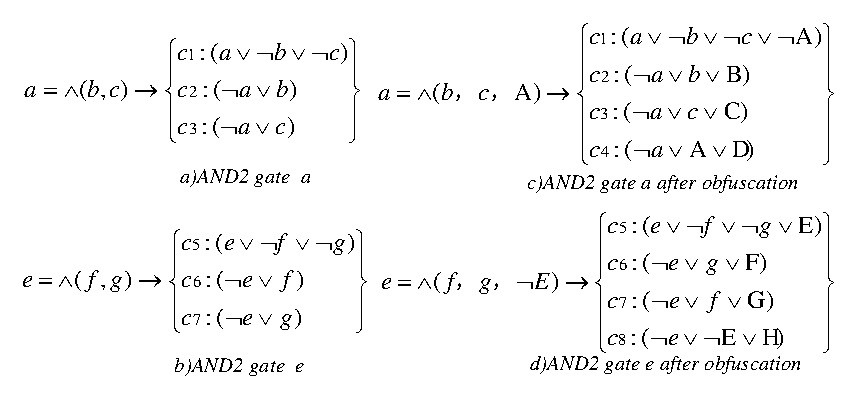
\includegraphics[width=8.2cm]{AND2-2}
\caption{混淆前后$a$和$e$的CNF标记}
%\caption{CNF signature of $a$ and $e$ before and after obfuscation}
\label{3:fig_beforeafter}
\end{figure}

图\ref{3:fig_beforeafter}a)和\ref{3:fig_beforeafter}b)给出了两个AND2门$a$和$e$CNF标记,
混淆后的标记显示在图\ref{3:fig_beforeafter}c)和\ref{3:fig_beforeafter}d)中。

有三种改变
\begin{enumerate}
 \item
 关键子句$c_1$和$c_5$ 的长度由3变为4,
基于关键子句模式匹配的电路结构探测算法\cite{csFu}将不再有效;
 \item
$a$的特征子句$c_1$-$c_3$)以及$e$的特征子句$c_5$-$c_7$变为了不同的形式,
并且有新的子句加入了公式如$c_4$和$c_8$,
基于标记子图同构的电路结构检测算法\cite{csRoy}将不再有效;
\item
 通过加入合适的新文字以及构造新的子句,
 门$a$ 的CNF标记从AND2变为了AND3,
如图\ref{3:fig_beforeafter}a)和\ref{3:fig_beforeafter}c)。
Husk文字$A$,
成为了新生成的AND3门的一个输入,
并且与原始AND2门的输入$b$和$c$不可区分。
这也使得区分混淆后AND2和真实AND3变得不再可能。
\end{enumerate}

\subsubsection{算法复杂性分析}
根据本章提出的基于混淆的SAT求解框架,SAT问题求解开销包含私有云上的计算开销和公共云中的计算开销。
在私有云中,计算开销包括CNF公式混淆开销和结果恢复开销;
在公共云中的计算开销是指对混淆后CNF公式的SAT 求解开销。
由于Husk公式可以预先产生,因此在本文中,Husk公式的产生开销不列入到一次SAT求解的开销。

\textbf{混淆算法的复杂性}

%Obfuscation is implemented in Algorithm \ref{3:algo_obs}.
%The main procedure of Algorithm \ref{3:algo_obs} consists only one layer of loop,
%but one of it sub-procedure $\mathbf{mark}$ (Algorithm \ref{3:algo_mark}) consists 4 layers of loop,
%and the runtimes of the 2 inner loops are bounded by length of clauses.
%So the complexity of the obfuscation algorithm is $O(n^2)$.
算法\ref{3:algo_obs}实现了混淆,其中主程序仅仅包含一层循环,
但是其中一个子程序$\mathbf{mark}$(算法\ref{3:algo_mark})包含了4层循环,
由于两层内循环的上界为子句长度,
因此混淆算法复杂性为$O(n^2)$。

\textbf{解恢复算法的复杂性}

%Solution recovery is implemented in  Algorithm \ref{3:algo_map},
%which only consists one layer of loop,
%its complexity is $O(n)$.
%According to Theorem \ref{3:SSOtheorem}, result from SAT solver may consist false solution,
%so Algorithm \ref{3:algo_map} may be run more than one time to get correct solution.
%Since Algorithm \ref{3:algo_map} is of linear complexity,
%it incurs minor impact on performance of SAT Solving.
解恢复在算法\ref{3:algo_map}中实现,
由于仅仅包含一层循环,算法复杂度为$O(n)$。
%根据定理\ref{3:SSOtheorem}, 来自于SAT求解器的解可能包含假解,
%因此为获得正确解,算法\ref{3:algo_map}可能会运行不只一次.
由于算法\ref{3:algo_map}为线性复杂度,
带给整个求解过程的开销较小。

\subsection{实验评估}
\subsubsection{实验设计}
本文给出的算法由C语言实现。
实验用机器的配置为Intel Core(TM) i7-3667U CPU @ 2.00GHz, 8GB RAM。

将ISCAS89测试集中的部分电路按照形式化验证时的要求分别展开20、30、100次并编码为CNF公式,
产生的Husks公式包含了节点数和子句数为$vn=675$/$cn=2309$,
使用本章给出的混淆算法和解映射算法,
使用MiniSat作为求解器,
模拟开放环境下隐私保护SAT求解计算。

\subsubsection{实验结果分析}
表\ref{3:fig_exp}给出了实验结果,表中各个参数的意义如下所示。 \\
$~~$\textbf{变量数/子句数(vn/cn)}:原始CNF 公式中的包含的变量数和子句数。\\
%$~~$\textbf{Marked Gate}:混淆过程中改变的门数。\\
$~~$\textbf{求解时间(Solving Time)}:混淆前后的SAT问题得到第一个可满足解的时间。\\
$~~$\textbf{混淆时间(Obfuscation Time)}:按照混淆算法在原公式中混合入HUSK公式的时间。\\
$~~$\textbf{解恢复时间(Map Time)}:从混淆后的解中恢复出实际解的时间。

实验证实了算法的正确性,对取自ISCAS89中的13个示例电路生成的可满足CNF公式,混淆前后的SAT求解的解一致。

就异构加速比( Asymmetric~Speedup)\cite{c.WANG}而言,100\%的电路, 加速比超过了100\%,特别是某些尺寸较大的电路,异构加速比超过500%
这表明了外包复杂SAT求解函数的必要性。
\begin{equation}
%异构加速比= \frac{求解时间}{混淆时间 + 解恢复时间}
Asymmetric~Speedup= \frac{Solving~Time}{Obfuscation~Times + Map~Time}
\end{equation}

实验也显示出混淆后带来的SAT求解的开销,不同的电路具有不同的表现。
\begin{equation}
%求解开销=\frac{混淆后求解时间-混淆前求解时间}{混淆前求解时间}
Solving~OverHead=\frac{Solving~Time~After~Obfuscation-Solving~Time~Before~Obfuscation}{Solving~Time~Before~Obfuscation}
\end{equation}
90\% 以上的电路,开销小于100\%,仅有少部分电路,开销超过了100\%;
表明简单的混淆策略引入的求解开销是可以接受的
%这些事实提醒我们两件事情:
%首先,混淆时间取决于被改变的门数,
%需要研究更加精巧的混淆算法以改变较少的门的情况下仍然可以迷惑攻击者.
%第二, 由于混淆引入的SAT求解开销,因电路而异,在设计混淆算法时,需要考虑修改后结构对求解时间的影响。

\begin{table*}
\caption{不同类型电路CNF公式混淆前后的运行时间}
%\caption{Runtime of CNF formula generated from different Circuit}
\centering
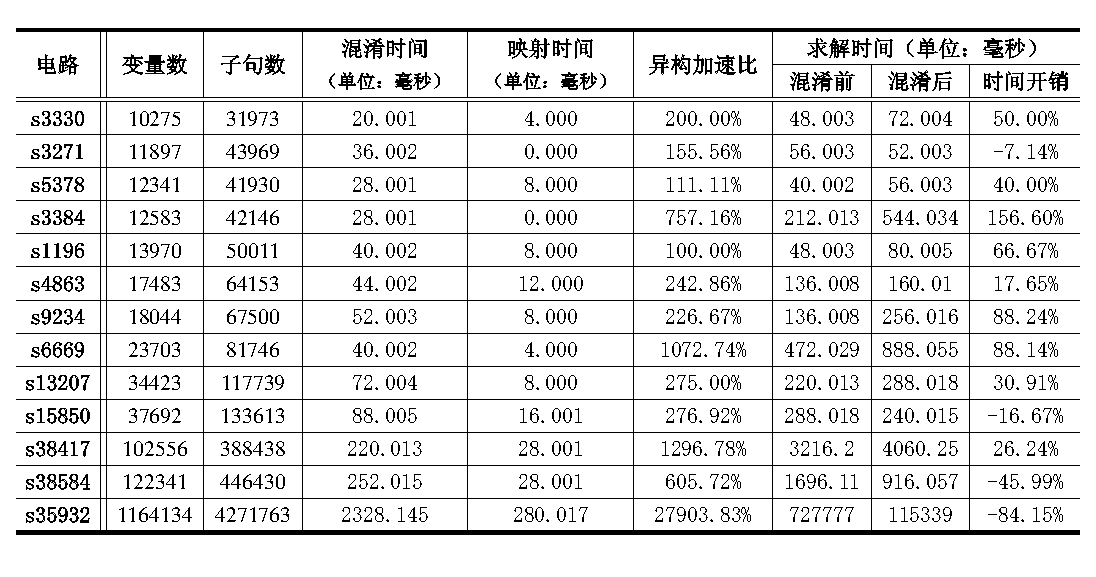
\includegraphics[width=14.2cm]{fig302}
\label{3:fig_exp}
\end{table*}%
%
%\section{Conclusion}
%This paper proposes a circuit aware  CNF obfuscation algorithm,
%that can prevent the confidential information from being recovered by adversary,
%when outsourcing SAT problem in Cloud or grid.
%Theoretical analysis and experimental results show that algorithms can significantly change structure of CNF formula,
%with polynomial complexity and without narrowing down its solution space.
\section{本章小结}
在本章中,我们对SAT求解的安全外包进行了建模,
给出了实现SAT问题求解输入隐私保护的有效方案。
设计了结构感知的CNF混淆方法,
可以防止敏感的输入信息如电路结构被恢复。
理论和实验结果都证明了方案的实用型。
%本文给出了电路结构感知的CNF混淆算法,可防止在SAT问题外包计算时,CNF公式中的电路结构以及解被窃取。
%理论分析和实验表明,算法可以有效的改变结构,同时还不会缩减CNF公式的解空间。
